\documentclass{article}
\usepackage[utf8]{inputenc}
\setlength{\oddsidemargin}{-0.2in}
\setlength{\evensidemargin}{0.2in}
\setlength{\textwidth}{6.5in}
\setlength{\textheight}{9.5in}
\setlength{\topmargin}{-0.75in}
\usepackage{authblk}
\usepackage{amsmath}
 \usepackage{todonotes}
\usepackage{graphicx}
 \usepackage{setspace}
\doublespacing
\usepackage[style=numeric]{biblatex}
  

\addbibresource{references.bib}




  
      

       \title{Modelling Exciton Diffusion - Final Report}

       
            
       \vspace{1.5cm}
       
       \author{Alfy Benny, Kipp Bradford, Savannah Carnahan,\\ Xiaoqi Chen, and Azmaine Iqtidar}
        \begin{document}
       \maketitle
      
       \vfill
            
       
            
      \vfill
     
       \begin{center}
            
       Software Engineering in Scientific Computing\\
       Princeton University\\
       
    \end{center}    
  
\newpage

\tableofcontents %Added this


\section{Introduction}

\subsection{Motivation}

Designing, predicting and understanding energy transport in opto-electronic devices and biological systems is a major challenge facing materials science and biology. Exciton transport is a fundamental mode of energy transfer in such systems. Excitons are formed when an electron is excited from its ground state into the conduction band of the material. The exciton is then defined as the quasi-particle formed by the excited electron and the positive hole it left behind. Once an exciton is formed on one molecule, it can then then diffuse to other particles in the system. 

There are two well-established methods for modelling exciton transport.\cite{Oberhofer2017ChargeMethods} In the hopping regime, the particle is viewed as discretely localized on a site in the material. The exciton can then jump from one site to another with a probability depending on the system in question. This approach is best suited to highly disordered materials due to Andersen delocalisation and polaron formation.\cite{DanielBalzer2021DelocalisedMaterials}

In highly ordered materials, the exciton is best modelled as a wave because in these materials the exciton can exist delocalized over several sites.\cite{Oberhofer2017ChargeMethods} It is therefore inaccurate to model the exciton dispersion as existing on discrete sites, and thus, the mobility of the exciton in the material is instead modelled using the velocity of the wavepacket. These two models are quite successful at modelling transports at the extremes; however, many modern materials are in an intermediate zone that is not well described by either model. There are several models that aim to bridge the gap between the models, called the intermediate regime. Our software will primarily focus on modelling the hopping regime, with the goal of having the flexibility to accommodate further advances in models in the field, particularly complications that arise in the intermediate regime.

\subsection{Theory}

The mechanism of charge transport, regardless of classification is governed by the conductivity of the material $\sigma$:
\begin{align}
    \mathbf{\sigma}=&q\rho_c\mathbf{\mu}
\end{align}

where $q$ is the charge, $\rho_c$ is the density of carriers, and $\mathbf{\mu}$ corresponds to the likelihood that that charge will move in the material (i.e its mobility).\cite{Oberhofer2017ChargeMethods} Both $\mathbf{\mu}$ and $\rho_c$ are dependent on the system being examined. This project is primarily concerned with determining $\mathbf{\mu}$ for a given material with density $\rho_c$. 

In the hopping regime, the probability that an exciton will transfer from site 1 to site 2 is governed in the nonadiabatic limit by the Marcus rate equation:\cite{Marcus1956OnIN}
\begin{align}
    k_{12,nadiab}=&\frac{2\pi}{\hbar}|J_{Coul}|^2\sqrt{\frac{1}{4\pi k_b T \lambda}}e^{-\frac{(\lambda +\Delta G^0)^2}{4\lambda k_b T}}
\end{align}

where $\hbar$ and $k_b$ are constants, $\lambda$ is the reorganization free energy, $J_{Coul}$ is the coupling between the initial site and final site, $\Delta G^0$ is the driving force, and $T$ is the temperature. In the adiabatic limit, this is defined by the Arrhenius equation:\cite{Baumeier2012StochasticNetworks}

\begin{align}
    k_{12,adiab}=&\mu_{eff}e^{-\beta(\Delta G^{\ddag}-\Delta^\ddag)}
\end{align}

A yet another widely used formula to calculate the rate, in the context of Förster resonance energy transfer (FRET) is as follows:-

\begin{align}
    k_{12,FRET}=&\frac{2\pi}{\hbar}\frac{1}{(4\pi\epsilon_0)^2} \frac{\kappa^2|\mu_1|^2|\mu_2|^2}{r^6}Q_DSpectralOverlap
\end{align}
Where $\kappa$ is the orientation factor, $\mu_1$ and $\mu_2$ are the transition dipoles on site 1 and 2, respectively, r is the distance between the chromophores, and \textit{SpectralOverlap} is the overlap between absorption and emission spectra of site2 and site1, respectively. 

Therefore the movement of the exciton through the material can be modelled using the kinetic Monte Carlo (kMC) method.\cite{Oberhofer2017ChargeMethods} Beginning at $t=0$, the algorithm is propagated with a chosen time step. The probability that a charge localized at site 1 will jump to one of $i$ sites it is connected to is governed by the summation of the transition rates:
\begin{align}
    K_{12}=&\sum_{j=2}^{i+1} k_{1j}
\end{align}

A random number between $0$ and $K_{12}$ is chosen as the probability $p$, and the site $2$ to be transitioned to depends on where in the interval $p$ falls. When this event occurs is determined by the time-dependent distribution:
\begin{align}
    p_{12}(t)=k_{12}e^{k_{12}t}
\end{align}
Once the exciton is transferred, the process is repeated for a predetermined number of steps or until a total simulation time $\tau$ is reached. 
Once the simulation is complete, the mobility $\mathbf{\mu}$ is determined by averaging over the kMC trajectories.
\begin{align}
    \mathbf{\mu}=&\frac{\langle \mathbf{v}\rangle}{\mathbf{E}}\\
    \langle\mathbf{v}\rangle=&\frac{\mathbf{R}_{final}-\mathbf{R}_{initial}}{\tau}
\end{align}


\subsection{Proposed Project}

We propose to create a flexible tool to examine exciton diffusion in a variety of materials. The tool will initially only support materials in the hopping regime but would have the flexibility to extend to more complicated equations that describe the intermediate regime. The project will begin by examining point particles and will then expand to include more physical systems, such as atoms in a crystal lattice.

\section{Design}

The software will implement a factory design pattern so that it can be easily expanded to accommodate more methods and models. The general outline of the software is as follows:

\begin{itemize}
    \item Input is taken from the user in the form of either the name of a text file, a model, and a system type or just the name of a model.
    \item According to the input of model and system, the ModelFactory and the SystemFactory initialize a model and a system, respectively.
    \item The System excites molecules according to a prescribed method.
    \item The Model is run on the system to calculate the diffusion distance of the exciton for a given period.
    \item The Model output is shown in the form of a graphical representation of the exciton path (or the longest exciton path) of the system.
\end{itemize}

\begin{figure}
    \centering
   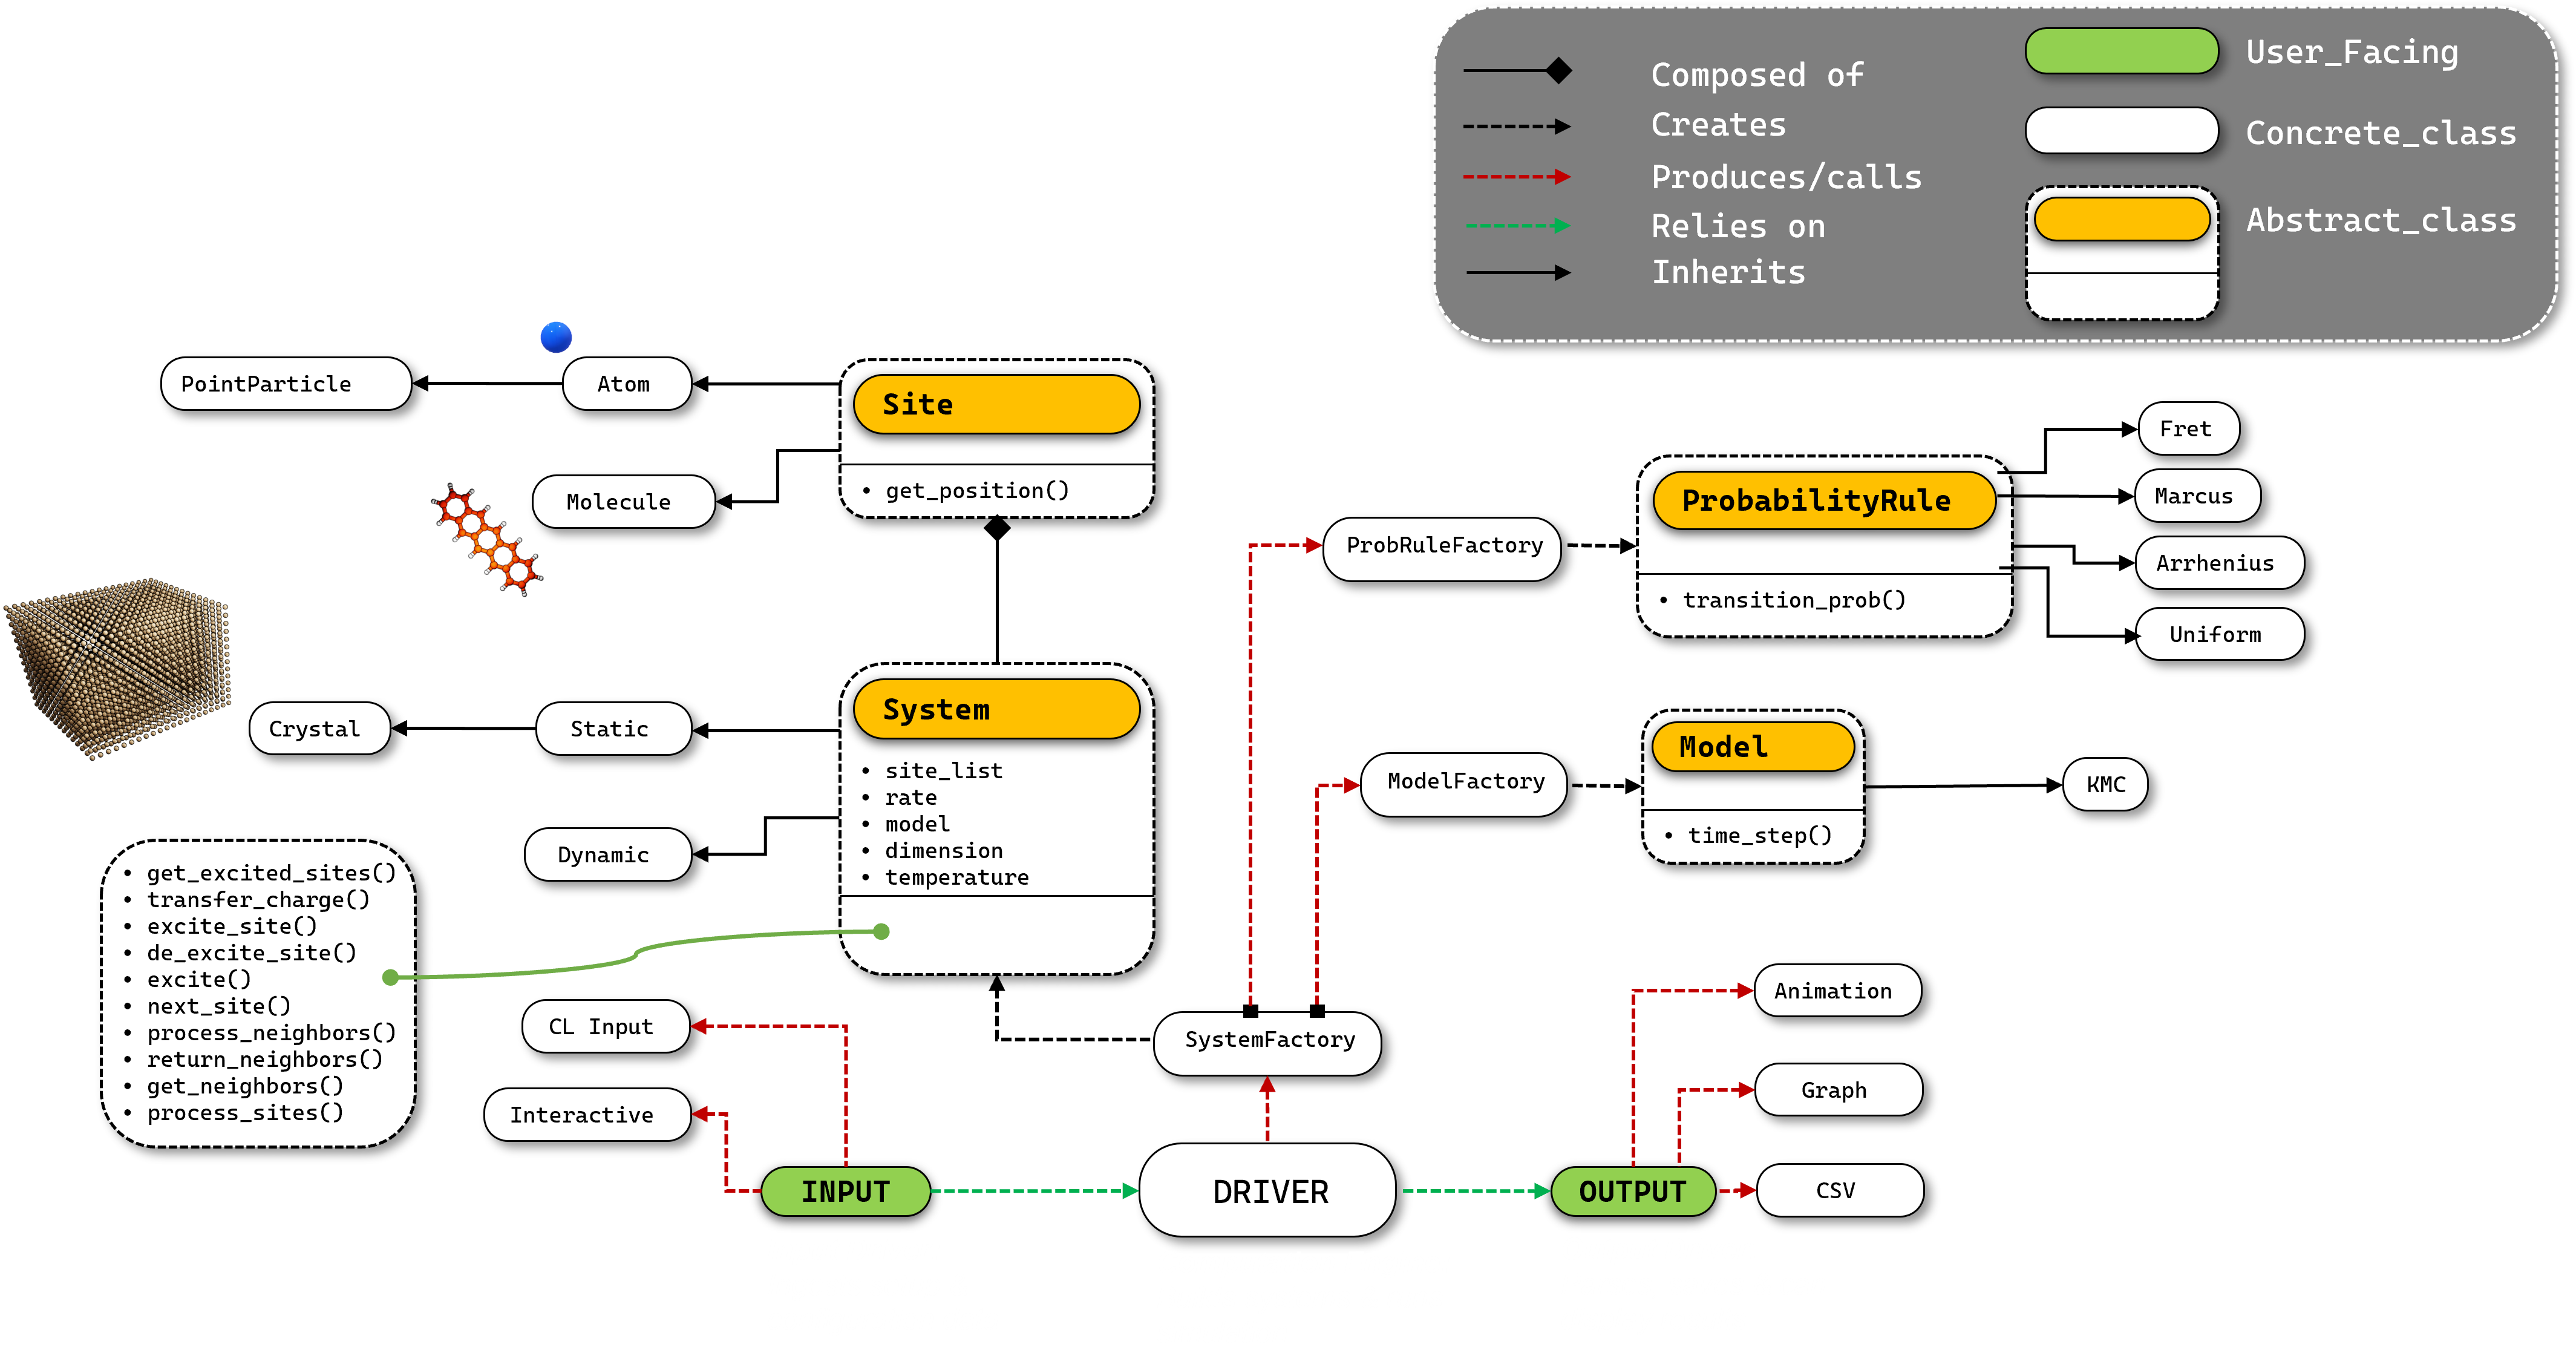
\includegraphics[scale=0.4]{UML_2.png}
    \caption{UML Diagram}
    \label{fig:my_label}
\end{figure}



\subsection{Input}




\subsection{Factories}

\subsubsection{Site Factory}

\subsubsection{System Factory}

\subsubsection{Model Factory}

\subsubsection{Probability Rule Factory}




\subsection{Primary Algorithm}




\subsection{Sites}

A site's most important attribute is the boolean value excited, which returns true if the site is excited and false otherwise. It also contains several attributes that aid in the calculation of probability rules. Every site 

\subsubsection{Atom and PointParticle}

\subsubsection{Molecule}

\subsection{System}

Any instance of the abstract System class will be an aggregate class of sites. These sites all have position, and the aggregate classes keep track of which particles are close to each other. Additionally, the abstract System class will contain a method to excite sites randomly based on either charge density or a random selection process (depending on the presence of single or multiple excitons). Currently, implemented sub-classes are Static and Crystal, both of which are characterized by non-moving sites. A future subclass is Dynamic, which would be 

\subsubsection{System Attributes}

The two most important System attributes are model, which corresponds to a Model object, and rate, which corresponds to a Probability Rule object. Both of these objects are utilized 

\subsubsection{System Methods}

\subsection{Model}

The model is an abstract base class for objects responsible for advancing the system forward by one step. It is also responsible for selecting the next site given a list of sites and rates. It also calculates how much time the step takes given two sites and a system. The time step method returns a change in time.

\subsubsection{Subclasses}

Currently, the only model implemented is the kinetic Monte Carlo. It selects the next site by adding up the rates of possible transfer sites, choosing a random number between 0 and the sum, and selecting the next site based on where that number falls. Essentially, if the rate of transfer corresponds to $k_{1b}$, where $b$ is an index representing the number of the possible transfer sites, if the random number falls between 0 and $k_{12}$, site 2 is selected, if it is between $k_{12}$ and $k_{12}+k_{13}$, site 3 is selected, etc. Once a site A is selected, the time advancement is determined by a random number from an exponential distribution based on the rate $k_{1A}$.

\subsection{Probability Rules}

Probability rules are responsible for returning coupling rates based on the system under examination and two site objects. The transition probability method returns a float representing the numerator of a probability. 



\subsubsection{Hamiltonian}

The Hamiltonian method is used by all the probability rules. Its calculation does not change based on the probability rule, and therefore lives in the abstract base class.



\subsubsection{Types of Rules}

The subclasses FRET, Arrhenius, and Marcus run these calculations based on equations 2, 3, and 4 respectively. The Uniform subclass just returns 1, corresponding to a uniform probability distribution when normalized.


\subsection{Output}
Apart from providing on-screen real time text output of progress as the exciton propagates through the system, our libraries currently support three forms of output: Text, Graphs and Animation.

\subsubsection{Text}
Data encoding the excited states over time can be saved in the form of a CSV file. This allows for the data to be saved and processed later on without re-running the entire simulation.
\subsubsection{Graphs}
Built-in functions also enable the creation of:

\begin{enumerate}
    \item 3D-plots of any system state, given the appropriate parameters, with the excitons marked in the plot by a different color. 
    \item 2D-plots of the propagation of the diffusion distance with time. This information carries theoretical value in understanding the behavior of the model in terms of its parameters.
\end{enumerate}
\subsubsection{Animation}
3D-animations of the exciton propagation through the system can also be created. These animations follow a similar pattern to the 3D-plots of the system, with the entire system being recreated and the excitons at any one time being marked with a different color. These animations can be played in real-time and/or saved at a directory of choice for later viewing. \todo{Insert an animation picture here}


\begin{figure}
    \centering
   \includegraphics[scale=.35]{out2.png}
    \caption{Exciton transport visualization}
    \label{fig:my_label}
\end{figure}

\section{Development Process}

\subsection{Planned Workflow}

\subsection{Continuous Integration Testing}

\subsection{Workflow Hiccups}

\subsection{Design Mistakes and Fixes}



\section{Profiling}

\subsection{Results}

\subsection{Improvements}




\section{Future Improvements}





\printbibliography

\end{document}  